\documentclass[12pt]{article}
\usepackage[utf8]{inputenc}
\usepackage[T1]{fontenc}
\usepackage{graphicx}
\usepackage{xcolor}

%%novalidate

\usepackage{tikz}
\usepackage{calc}
\usepackage{booktabs}


% colors
\definecolor{color1}{HTML}{000060}
%\definecolor{color1}{HTML}{8C260F}
\definecolor{color2}{HTML}{333333}


% fonts
\usepackage{fontspec}
\defaultfontfeatures{Mapping=tex-text}
\setmainfont
[BoldFont=Lato-Bold.ttf,
ItalicFont=Lato-Italic.ttf,
BoldItalicFont=Lato-BoldItalic.ttf]
{Lato-Regular.ttf}
\newfontfamily\headingfont[ItalicFont=Lato-BlackItalic.ttf]{Lato-Black.ttf}
%%%

\usepackage{geometry}
\geometry{a4paper,
hmargin=20mm,vmargin=20mm,
head=0ex,foot=3ex}

\linespread{1.3}

\usepackage[hang]{caption}
\DeclareCaptionFormat{upper}{#1#2\uppercase{#3}\par}
\captionsetup{labelfont={bf,color=color2},textfont={normalsize,color=color2},format = upper,figurename=FIGURE,tablename=TABLE}

%%% fancy sections
\usepackage{titlesec}
%\titleformat{\chapter}{\headingfont\LARGE\bfseries\scshape\color{color1}}{\thechapter}{1em}{}[\titlerule]
\titleformat{\section}{\color{color1}\headingfont\Large\bfseries\uppercase}{\thesection}{1em}{}[\titlerule]
\titleformat{\subsection}{\color{color1}\headingfont\large\bfseries\uppercase}{\thesubsection}{1em}{}
\titleformat{\subsubsection}{\color{color1}\headingfont\bfseries\uppercase}{\thesubsubsection}{1em}{}
%%%

% head and foot
\usepackage{fancyhdr}
\pagestyle{fancy}
\lhead{}
\chead{}
\makeatletter
\rhead{\color{color2}\@date}
\makeatother
\newlength{\myheight}
\lfoot{
\settoheight{\myheight}{\thepage}
\raisebox{-2ex-0.5\myheight}{
\includegraphics[height=4ex]{logo}}
}
\cfoot{\color{color2}\ APC3}
\rfoot{\color{color2}\thepage}
\renewcommand\headrulewidth{0pt}
\renewcommand\footrulewidth{0pt}

% custom titlepage
\makeatletter
\newcommand*\DefVar[1]{\@namedef{#1}##1{\global\@namedef{get#1}{##1}}}
\DefVar{summary}
\renewcommand{\maketitle}{
\begin{center}

\begin{tikzpicture}
    \node[draw=none,%color1,line width=0.4pt,
      fill=color1,
      inner sep = 10pt,
      text width=\textwidth-20pt,
      text centered
    ] {\color{white}\headingfont\bfseries\huge\@title};
\end{tikzpicture}
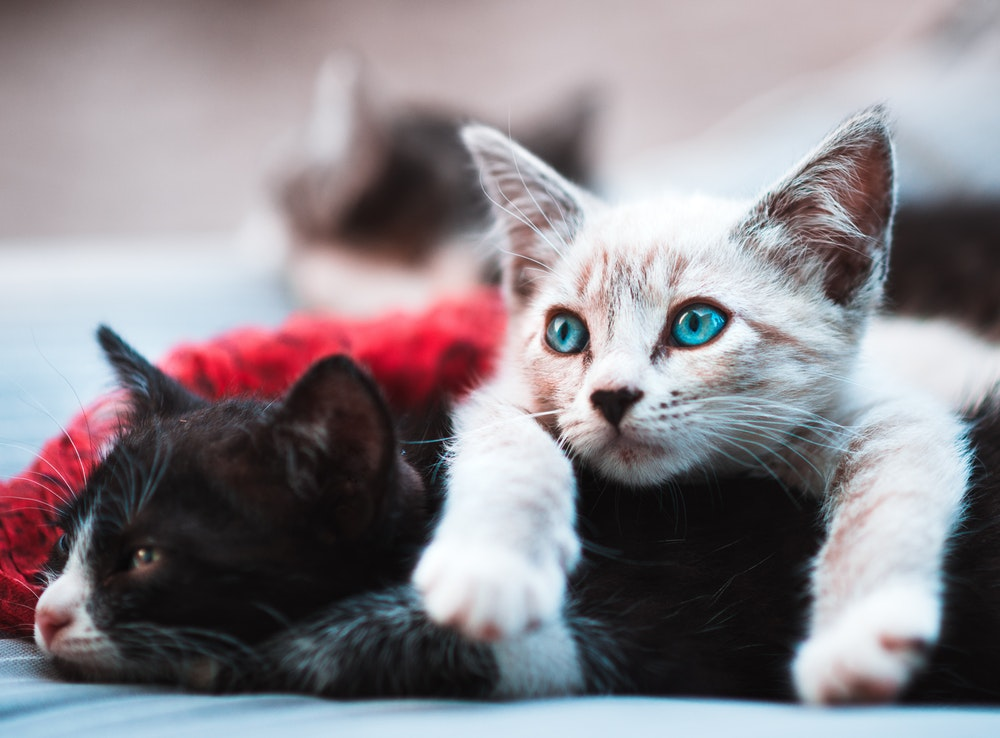
\includegraphics[width=\textwidth]{opening}\par
\headingfont\bfseries\Large\@author\par
\bigskip\medskip
{\color{color2}\normalfont\normalsize\textbf{Summary:}\\
\getsummary}
\end{center}
\clearpage
}
\makeatother
%%%

%%% fancy boxes
\usepackage{tcolorbox}
\usepackage{wrapfig}
\def\fullboxbegin{
\bigskip
\begin{tcolorbox}[colback=color1,colframe=color1,coltext=white,arc=0mm,boxrule=0pt]
}
\def\fullboxend{\end{tcolorbox}\medskip}
%
\def\leftboxbegin{
\begin{wrapfigure}{l}{0.5\textwidth}
\begin{tcolorbox}[colback=color1,colframe=color1,coltext=white,arc=0mm,boxrule=0pt]
}
\def\leftboxend{
\end{tcolorbox}
\end{wrapfigure}
}
%
\def\rightboxbegin{
\begin{wrapfigure}{r}{0.5\textwidth}
\begin{tcolorbox}[colback=color1,colframe=color1,coltext=white,arc=0mm,boxrule=0pt]
}
\def\rightboxend{
\end{tcolorbox}
\end{wrapfigure}
}
%
\newcounter{frames}
\def\frameboxbegin#1{
\bigskip
\refstepcounter{frames}
\begin{tcolorbox}[colback=white,colframe=color1,arc=0mm,title={\MakeUppercase{\textbf{Frame \arabic{frames}}: #1}}]
}
\def\frameboxend{
\end{tcolorbox}
}
%%%

\usepackage{lipsum}

%%%%%%%%%%%%%%%
% Title Page
\title{APC3 Assignment}
\author{Phoebe Liang}
\date{\today}
\summary{
Actuarial consultant providing advice to a general insurance company XYZ, which writes motor vehicle, home and contents, and building insurance policies. XYZ is expanding its policy offerings with a new product, electricity blackout insurance (EBI), to be made available to retail and commercial customers in Victoria. The committee is seeking advise on how this product would be structured and how it would be received by the customers. Furthermore, as part of its risk management strategy, the risk committee of XYZ is seeking advice in the use of electricity derivatives, so that they can report to the board on the feasibility of offering an electricity blackout insurance product.
}
%%%%%%%%%%%%%%%

\begin{document}
\maketitle

\tableofcontents
\clearpage

\section{Background}
\subsection{Electricity blackout Compensation}
\begin{flushleft}
start section here
\end{flushleft}

\subsection{Electricity Blackouts in Victoria}
\begin{flushleft}
start section here
\end{flushleft}

\subsection{Electricity market in Australia}
\begin{flushleft}
Give a background to the Australian electricity market, explaining how electricity is generated by providers, sent to the grid and dispatched to customers. \par
https://www.energy.vic.gov.au/safety-and-emergencies/power-outages/customer-compensation 
\end{flushleft}


\newpage


\section{Product Structure}
\begin{flushleft}
Explain what EBI would seek to achieve for XYZ and its customers, describing a potential 
structure for the product and explaining the likelihood and severity of electricity blackouts in Victoria.
https://www.canstar.com.au/news-articles/power-outages-covered-home-insurance/ \par
Household: Food, AC, alarms? Can you make claims under the current policy? \par
Commercial: Loss of sales/efficiency, impact on bottom line? How to quantify these? Spike in electricity prices?\par
What are coverages? What can be claimed? How long?  
\end{flushleft}

\fullboxbegin
blor
\fullboxend

\section{Pricing and Risk}
Describe how the proposed product could be priced and the risks for the insurer XYZ. 

\leftboxbegin
formular in here?
\leftboxend

\lipsum[1]

\rightboxbegin
\begin{itemize}
 \item Lorem ipsum
 \item Lorem ipsum
\end{itemize}
\rightboxend

\lipsum[1]

\subsection{Pricing}
\lipsum[1]

\subsection{Risk}
\lipsum[1]


\section{Relevant Derivatives}
Outline the relevant derivative products offered on the Australian Stock Exchange, including how they are quoted and priced, paying particular attention to futures and options in respect of: 
\begin{itemize}
 \item Base - Quarterly
 \item Base - Monthly
 \item Base - Caps
 \item Base - Strip
 \item Peak - Quarterly
\end{itemize}

\begin{figure}[!h]
\centering
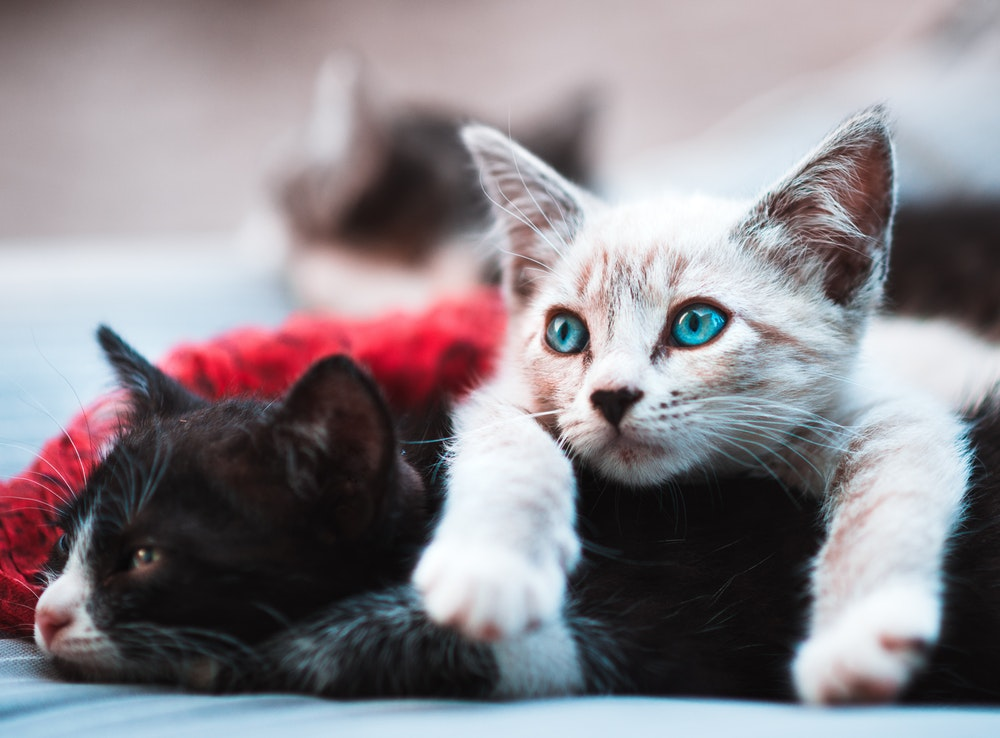
\includegraphics[width=0.5\textwidth]{opening.jpg}
\caption*{The sky is the limit.}
\end{figure}

\begin{table}[!h]
\centering
\caption{Sample table.}
\begin{tabular}{cccc}
\toprule
Value 1 & Value 2 & Value 3 & Value 4\\
\midrule
 odd     & odd   & odd & 1.00 \\
 even    & even  & even& 1.00 \\
 odd     & odd   & odd & 1.00 \\
 even    & even  & even& 1.00 \\
\bottomrule
\end{tabular}
\end{table}

\section{Liabilities Management}
Indicate how these could be used to manage XYZ’s EBI liabilities, giving a simple numerical example. \par

\frameboxbegin{Example: using derivatives to manage liabilities}
give a numerical example
\frameboxend


\section{Residual Risks Management}
Give some residual risks for XYZ and indicate how they could be managed. 

\section{Conclusion}
Give a conclusion on whether it is worthwhile XYZ pursuing an EBI offering, in whatever form. 

\end{document}          
